%% LaTeX Beamer presentation template (requires beamer package)
%% see http://latex-beamer.sourceforge.net/
%% idea contributed by H. Turgut Uyar
%% template based on a template by Till Tantau
%% this template is still evolving - it might differ in future releases!

\documentclass{beamer} 

%% ODER: format ==         = "\mathrel{==}"
%% ODER: format /=         = "\neq "
%
%
\makeatletter
\@ifundefined{lhs2tex.lhs2tex.sty.read}%
  {\@namedef{lhs2tex.lhs2tex.sty.read}{}%
   \newcommand\SkipToFmtEnd{}%
   \newcommand\EndFmtInput{}%
   \long\def\SkipToFmtEnd#1\EndFmtInput{}%
  }\SkipToFmtEnd

\newcommand\ReadOnlyOnce[1]{\@ifundefined{#1}{\@namedef{#1}{}}\SkipToFmtEnd}
\usepackage{amstext}
\usepackage{amssymb}
\usepackage{stmaryrd}
\DeclareFontFamily{OT1}{cmtex}{}
\DeclareFontShape{OT1}{cmtex}{m}{n}
  {<5><6><7><8>cmtex8
   <9>cmtex9
   <10><10.95><12><14.4><17.28><20.74><24.88>cmtex10}{}
\DeclareFontShape{OT1}{cmtex}{m}{it}
  {<-> ssub * cmtt/m/it}{}
\newcommand{\texfamily}{\fontfamily{cmtex}\selectfont}
\DeclareFontShape{OT1}{cmtt}{bx}{n}
  {<5><6><7><8>cmtt8
   <9>cmbtt9
   <10><10.95><12><14.4><17.28><20.74><24.88>cmbtt10}{}
\DeclareFontShape{OT1}{cmtex}{bx}{n}
  {<-> ssub * cmtt/bx/n}{}
\newcommand{\tex}[1]{\text{\texfamily#1}}	% NEU

\newcommand{\Sp}{\hskip.33334em\relax}


\newcommand{\Conid}[1]{\mathit{#1}}
\newcommand{\Varid}[1]{\mathit{#1}}
\newcommand{\anonymous}{\kern0.06em \vbox{\hrule\@width.5em}}
\newcommand{\plus}{\mathbin{+\!\!\!+}}
\newcommand{\bind}{\mathbin{>\!\!\!>\mkern-6.7mu=}}
\newcommand{\rbind}{\mathbin{=\mkern-6.7mu<\!\!\!<}}% suggested by Neil Mitchell
\newcommand{\sequ}{\mathbin{>\!\!\!>}}
\renewcommand{\leq}{\leqslant}
\renewcommand{\geq}{\geqslant}
\usepackage{polytable}

%mathindent has to be defined
\@ifundefined{mathindent}%
  {\newdimen\mathindent\mathindent\leftmargini}%
  {}%

\def\resethooks{%
  \global\let\SaveRestoreHook\empty
  \global\let\ColumnHook\empty}
\newcommand*{\savecolumns}[1][default]%
  {\g@addto@macro\SaveRestoreHook{\savecolumns[#1]}}
\newcommand*{\restorecolumns}[1][default]%
  {\g@addto@macro\SaveRestoreHook{\restorecolumns[#1]}}
\newcommand*{\aligncolumn}[2]%
  {\g@addto@macro\ColumnHook{\column{#1}{#2}}}

\resethooks

\newcommand{\onelinecommentchars}{\quad-{}- }
\newcommand{\commentbeginchars}{\enskip\{-}
\newcommand{\commentendchars}{-\}\enskip}

\newcommand{\visiblecomments}{%
  \let\onelinecomment=\onelinecommentchars
  \let\commentbegin=\commentbeginchars
  \let\commentend=\commentendchars}

\newcommand{\invisiblecomments}{%
  \let\onelinecomment=\empty
  \let\commentbegin=\empty
  \let\commentend=\empty}

\visiblecomments

\newlength{\blanklineskip}
\setlength{\blanklineskip}{0.66084ex}

\newcommand{\hsindent}[1]{\quad}% default is fixed indentation
\let\hspre\empty
\let\hspost\empty
\newcommand{\NB}{\textbf{NB}}
\newcommand{\Todo}[1]{$\langle$\textbf{To do:}~#1$\rangle$}

\EndFmtInput
\makeatother
%
%
%
%
%
%
% This package provides two environments suitable to take the place
% of hscode, called "plainhscode" and "arrayhscode". 
%
% The plain environment surrounds each code block by vertical space,
% and it uses \abovedisplayskip and \belowdisplayskip to get spacing
% similar to formulas. Note that if these dimensions are changed,
% the spacing around displayed math formulas changes as well.
% All code is indented using \leftskip.
%
% Changed 19.08.2004 to reflect changes in colorcode. Should work with
% CodeGroup.sty.
%
\ReadOnlyOnce{polycode.fmt}%
\makeatletter

\newcommand{\hsnewpar}[1]%
  {{\parskip=0pt\parindent=0pt\par\vskip #1\noindent}}

% can be used, for instance, to redefine the code size, by setting the
% command to \small or something alike
\newcommand{\hscodestyle}{}

% The command \sethscode can be used to switch the code formatting
% behaviour by mapping the hscode environment in the subst directive
% to a new LaTeX environment.

\newcommand{\sethscode}[1]%
  {\expandafter\let\expandafter\hscode\csname #1\endcsname
   \expandafter\let\expandafter\endhscode\csname end#1\endcsname}

% "compatibility" mode restores the non-polycode.fmt layout.

\newenvironment{compathscode}%
  {\par\noindent
   \advance\leftskip\mathindent
   \hscodestyle
   \let\\=\@normalcr
   \(\pboxed}%
  {\endpboxed\)%
   \par\noindent
   \ignorespacesafterend}

\newcommand{\compaths}{\sethscode{compathscode}}

% "plain" mode is the proposed default.
% It should now work with \centering.
% This required some changes. The old version
% is still available for reference as oldplainhscode.

\newenvironment{plainhscode}%
  {\hsnewpar\abovedisplayskip
   \advance\leftskip\mathindent
   \hscodestyle
   \let\hspre\(\let\hspost\)%
   \pboxed}%
  {\endpboxed%
   \hsnewpar\belowdisplayskip
   \ignorespacesafterend}

\newenvironment{oldplainhscode}%
  {\hsnewpar\abovedisplayskip
   \advance\leftskip\mathindent
   \hscodestyle
   \let\\=\@normalcr
   \(\pboxed}%
  {\endpboxed\)%
   \hsnewpar\belowdisplayskip
   \ignorespacesafterend}

% Here, we make plainhscode the default environment.

\newcommand{\plainhs}{\sethscode{plainhscode}}
\newcommand{\oldplainhs}{\sethscode{oldplainhscode}}
\plainhs

% The arrayhscode is like plain, but makes use of polytable's
% parray environment which disallows page breaks in code blocks.

\newenvironment{arrayhscode}%
  {\hsnewpar\abovedisplayskip
   \advance\leftskip\mathindent
   \hscodestyle
   \let\\=\@normalcr
   \(\parray}%
  {\endparray\)%
   \hsnewpar\belowdisplayskip
   \ignorespacesafterend}

\newcommand{\arrayhs}{\sethscode{arrayhscode}}

% The mathhscode environment also makes use of polytable's parray 
% environment. It is supposed to be used only inside math mode 
% (I used it to typeset the type rules in my thesis).

\newenvironment{mathhscode}%
  {\parray}{\endparray}

\newcommand{\mathhs}{\sethscode{mathhscode}}

% texths is similar to mathhs, but works in text mode.

\newenvironment{texthscode}%
  {\(\parray}{\endparray\)}

\newcommand{\texths}{\sethscode{texthscode}}

% The framed environment places code in a framed box.

\def\codeframewidth{\arrayrulewidth}
\RequirePackage{calc}

\newenvironment{framedhscode}%
  {\parskip=\abovedisplayskip\par\noindent
   \hscodestyle
   \arrayrulewidth=\codeframewidth
   \tabular{@{}|p{\linewidth-2\arraycolsep-2\arrayrulewidth-2pt}|@{}}%
   \hline\framedhslinecorrect\\{-1.5ex}%
   \let\endoflinesave=\\
   \let\\=\@normalcr
   \(\pboxed}%
  {\endpboxed\)%
   \framedhslinecorrect\endoflinesave{.5ex}\hline
   \endtabular
   \parskip=\belowdisplayskip\par\noindent
   \ignorespacesafterend}

\newcommand{\framedhslinecorrect}[2]%
  {#1[#2]}

\newcommand{\framedhs}{\sethscode{framedhscode}}

% The inlinehscode environment is an experimental environment
% that can be used to typeset displayed code inline.

\newenvironment{inlinehscode}%
  {\(\def\column##1##2{}%
   \let\>\undefined\let\<\undefined\let\\\undefined
   \newcommand\>[1][]{}\newcommand\<[1][]{}\newcommand\\[1][]{}%
   \def\fromto##1##2##3{##3}%
   \def\nextline{}}{\) }%

\newcommand{\inlinehs}{\sethscode{inlinehscode}}

% The joincode environment is a separate environment that
% can be used to surround and thereby connect multiple code
% blocks.

\newenvironment{joincode}%
  {\let\orighscode=\hscode
   \let\origendhscode=\endhscode
   \def\endhscode{\def\hscode{\endgroup\def\@currenvir{hscode}\\}\begingroup}
   %\let\SaveRestoreHook=\empty
   %\let\ColumnHook=\empty
   %\let\resethooks=\empty
   \orighscode\def\hscode{\endgroup\def\@currenvir{hscode}}}%
  {\origendhscode
   \global\let\hscode=\orighscode
   \global\let\endhscode=\origendhscode}%

\makeatother
\EndFmtInput
%


% \mode<presentation>
% {
% \usetheme{Warsaw}
% 
% \setbeamercovered{transparent}
% }

\usetheme{CambridgeUS}
\usepackage[english]{babel}
\usepackage[latin1]{inputenc}


\title{A Haskell Library for Feature Modeling}

\author{Rodrigo Bonif\'{a}cio \and Paulo Borba}


\institute
{
	Informatics Center \\ Federal University of Pernambuco \\ Brazil
}


\begin{document}



\begin{frame}
\titlepage
\end{frame}

\begin{frame}
 \frametitle{Features}
 
 \begin{itemize}
  \item Feature models enriched with properties and global constraints
  \item Type and satisfiability checkers
  \item Integration with FMPlugin and FMIde
  \item Minnor points:
  \begin{itemize}
    \item Following the hackage structure
    \item Embedded in literate haskell--- is it good?
  \end{itemize} 
\end{itemize}
 
\end{frame}

\begin{frame}
\frametitle{Data types}
\begin{block}{Feature Model and Feature Configuration}
\begin{hscode}\SaveRestoreHook
\column{B}{@{}>{\hspre}l<{\hspost}@{}}%
\column{9}{@{}>{\hspre}l<{\hspost}@{}}%
\column{E}{@{}>{\hspre}l<{\hspost}@{}}%
\>[B]{}\mathbf{data}\;\Conid{FeatureModel}\mathrel{=}\Conid{FeatureModel}\;\{\mskip1.5mu {}\<[E]%
\\
\>[B]{}\hsindent{9}{}\<[9]%
\>[9]{}\Varid{fmRoot}\mathbin{::}\Conid{Root},{}\<[E]%
\\
\>[B]{}\hsindent{9}{}\<[9]%
\>[9]{}\Varid{fmConstraints}\mathbin{::}\Conid{Constraints}{}\<[E]%
\\
\>[B]{}\mskip1.5mu\}\;\mathbf{deriving}\;(\Conid{Show}){}\<[E]%
\\
\>[B]{}\mathbf{data}\;\Conid{FeatureConfiguration}\mathrel{=}\Conid{FeatureConfiguration}\;\{\mskip1.5mu {}\<[E]%
\\
\>[B]{}\hsindent{9}{}\<[9]%
\>[9]{}\Varid{fcRoot}\mathbin{::}\Conid{Root}{}\<[E]%
\\
\>[B]{}\mskip1.5mu\}\;\mathbf{deriving}\;(\Conid{Show}){}\<[E]%
\ColumnHook
\end{hscode}\resethooks
\end{block}

\end{frame}

\begin{frame}
\frametitle{Data types}
\begin{block}{Feature}
\begin{hscode}\SaveRestoreHook
\column{B}{@{}>{\hspre}l<{\hspost}@{}}%
\column{9}{@{}>{\hspre}l<{\hspost}@{}}%
\column{E}{@{}>{\hspre}l<{\hspost}@{}}%
\>[B]{}\mathbf{data}\;\Conid{Feature}\mathrel{=}\Conid{Feature}\;\{\mskip1.5mu {}\<[E]%
\\
\>[B]{}\hsindent{9}{}\<[9]%
\>[9]{}\Varid{fId}\mathbin{::}\Conid{Id},{}\<[E]%
\\
\>[B]{}\hsindent{9}{}\<[9]%
\>[9]{}\Varid{fName}\mathbin{::}\Conid{Name},{}\<[E]%
\\
\>[B]{}\hsindent{9}{}\<[9]%
\>[9]{}\Varid{fType}\mathbin{::}\Conid{FeatureType},{}\<[E]%
\\
\>[B]{}\hsindent{9}{}\<[9]%
\>[9]{}\Varid{groupType}\mathbin{::}\Conid{GroupType},{}\<[E]%
\\
\>[B]{}\hsindent{9}{}\<[9]%
\>[9]{}\Varid{children}\mathbin{::}\Conid{Children},{}\<[E]%
\\
\>[B]{}\hsindent{9}{}\<[9]%
\>[9]{}\Varid{properties}\mathbin{::}\Conid{Properties}{}\<[E]%
\\
\>[B]{}\mskip1.5mu\}\mid \Conid{FeatureError}{}\<[E]%
\ColumnHook
\end{hscode}\resethooks
\end{block}

\end{frame}

\begin{frame}
\frametitle{Data types}
\begin{block}{Global constraints}
\texttt{
\begin{hscode}\SaveRestoreHook
\column{B}{@{}>{\hspre}l<{\hspost}@{}}%
\column{9}{@{}>{\hspre}l<{\hspost}@{}}%
\column{E}{@{}>{\hspre}l<{\hspost}@{}}%
\>[B]{}\mathbf{data}\;\Conid{ConstraintType}\mathrel{=}\Conid{Implies}\mid \Conid{Iff}{}\<[E]%
\\
\>[B]{}\mathbf{deriving}\;(\Conid{Show}){}\<[E]%
\\[\blanklineskip]%
\>[B]{}\mathbf{data}\;\Conid{Constraint}\mathrel{=}\Conid{Constraint}\;\{\mskip1.5mu {}\<[E]%
\\
\>[B]{}\hsindent{9}{}\<[9]%
\>[9]{}\Varid{constraintType}\mathbin{::}\Conid{ConstraintType},{}\<[E]%
\\
\>[B]{}\hsindent{9}{}\<[9]%
\>[9]{}\Varid{constraintLHSExp}\mathbin{::}\Conid{FeatureExpression},{}\<[E]%
\\
\>[B]{}\hsindent{9}{}\<[9]%
\>[9]{}\Varid{constraintRHSExp}\mathbin{::}\Conid{FeatureExpression}{}\<[E]%
\\
\>[B]{}\mskip1.5mu\}\;\mathbf{deriving}\;(\Conid{Show}){}\<[E]%
\ColumnHook
\end{hscode}\resethooks
}
\end{block}

\end{frame}

\begin{frame}
\frametitle{Feature Model Type Checker}

\begin{enumerate}
 \item The root feature must be a mandatory feature
 \item Feature ids must be unique in a feature model
 \item All features must be well typed
 \item Feature options must be defined as optional
 \item The global constraints must be well typed
 \item The feature model must accept at least one instance
 \item \ldots
\end{enumerate}
\end{frame}

\begin{frame}
\frametitle{Feature Model Satisfiability}
\begin{block}{SAT solver for checking the FM constraints}
 \begin{itemize}
  \item Features translated to CNF expressions 
  \begin{itemize}
   \item Using the De Morgan's laws and distribution of $\land$ and $\lor$
   \item Using the Tseitin's transformation approach 
  \end{itemize}
  \item FUNSAT library used for verifying CNF satisfability
 \end{itemize} 
\end{block}
\end{frame}

\begin{frame}
\frametitle{Mapping Features into Propositional Logic}
\begin{hscode}\SaveRestoreHook
\column{B}{@{}>{\hspre}l<{\hspost}@{}}%
\column{3}{@{}>{\hspre}l<{\hspost}@{}}%
\column{4}{@{}>{\hspre}l<{\hspost}@{}}%
\column{5}{@{}>{\hspre}l<{\hspost}@{}}%
\column{11}{@{}>{\hspre}l<{\hspost}@{}}%
\column{24}{@{}>{\hspre}l<{\hspost}@{}}%
\column{E}{@{}>{\hspre}l<{\hspost}@{}}%
\>[B]{}\Varid{featureToPL}\;\Varid{f}\mathrel{=}{}\<[E]%
\\
\>[B]{}\hsindent{3}{}\<[3]%
\>[3]{}\mathbf{let}\;\Varid{cs}\mathrel{=}\Varid{children}\;\Varid{f}{}\<[E]%
\\
\>[B]{}\hsindent{3}{}\<[3]%
\>[3]{}\mathbf{in}{}\<[E]%
\\
\>[3]{}\hsindent{1}{}\<[4]%
\>[4]{}\mathbf{case}\;\Varid{groupType}\;\Varid{f}\;\mathbf{of}{}\<[E]%
\\
\>[4]{}\hsindent{1}{}\<[5]%
\>[5]{}\Conid{Basic}\to [\mskip1.5mu \Varid{f}\Rightarrow\Varid{c}{}\<[24]%
\>[24]{}\mid \Varid{c}\leftarrow \Varid{cs},\Varid{fType}\;\Varid{c}\equiv \Conid{Mandatory}\mskip1.5mu]{}\<[E]%
\\
\>[4]{}\hsindent{1}{}\<[5]%
\>[5]{}\Conid{IOR}{}\<[11]%
\>[11]{}\to [\mskip1.5mu \Varid{f}\Rightarrow(\Varid{foldOr}\;[\mskip1.5mu \Varid{ref}\;\Varid{c}\mid \Varid{c}\leftarrow \Varid{cs}\mskip1.5mu])\mskip1.5mu]{}\<[E]%
\\
\>[4]{}\hsindent{1}{}\<[5]%
\>[5]{}\Conid{XOR}{}\<[11]%
\>[11]{}\to [\mskip1.5mu \Varid{f}\Rightarrow(\Varid{foldOr}\;[\mskip1.5mu \Varid{xor}\;\Varid{c}\;(\Varid{delete}\;\Varid{c}\;(\Varid{cs}))\mid \Varid{c}\leftarrow \Varid{cs}\mskip1.5mu])\mskip1.5mu]{}\<[E]%
\ColumnHook
\end{hscode}\resethooks
\end{frame}

\begin{frame}
\frametitle{Benchmark for the satisfiability checker}

\begin{description}
 \item[CNF(FM100):] v = 381, c = 616
 \item[CNF(FM200):] v = 415, c = 663
 \item[CNF(FM500):] v = 988, c = 1587 
\end{description}
\begin{center}
 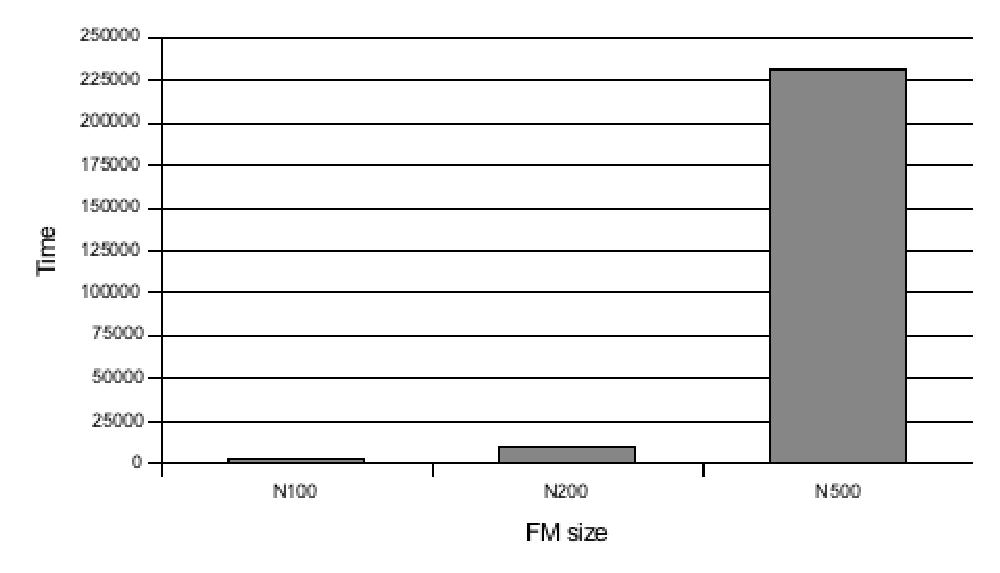
\includegraphics[scale=0.4]{images/bench.eps}
\end{center}
\end{frame}

\begin{frame}
\frametitle{Type Checker for Feature Configuration}
\begin{itemize}
 \item The related feature model (FM) must be well typed
 \item The selection of features must be an instance of FM 
\end{itemize}
\end{frame}

\begin{frame}
\frametitle{Type Checker for Feature Configuration}
\begin{block}{Interpreting both FM and FC}
\begin{hscode}\SaveRestoreHook
\column{B}{@{}>{\hspre}l<{\hspost}@{}}%
\column{3}{@{}>{\hspre}l<{\hspost}@{}}%
\column{4}{@{}>{\hspre}l<{\hspost}@{}}%
\column{6}{@{}>{\hspre}l<{\hspost}@{}}%
\column{E}{@{}>{\hspre}l<{\hspost}@{}}%
\>[B]{}\Varid{validInstance}\mathbin{::}\Conid{FeatureModel}\to \Conid{FeatureConfiguration}\to \Conid{ErrorList}{}\<[E]%
\\
\>[B]{}\Varid{validInstance}\;\Varid{fm}\;\Varid{fc}\mathrel{=}{}\<[E]%
\\
\>[B]{}\mathbf{let}\;\Varid{f1}\mathrel{=}\Varid{fmRoot}\;\Varid{fm}{}\<[E]%
\\
\>[B]{}\hsindent{6}{}\<[6]%
\>[6]{}\Varid{f2}\mathrel{=}\Varid{fcRoot}\;\Varid{fc}{}\<[E]%
\\
\>[B]{}\mathbf{in}{}\<[E]%
\\
\>[B]{}\hsindent{3}{}\<[3]%
\>[3]{}\mathbf{if}\;(\Varid{f1}\equiv \Varid{f2})\;\mathbf{then}\;(\Varid{checkType}\;\Varid{fm})\plus (\Varid{checkFeatures}\;\Varid{f1}\;\Varid{f2})\plus (\Varid{checkConstraints}\;\Varid{fm}\;\Varid{fc}){}\<[E]%
\\
\>[B]{}\hsindent{3}{}\<[3]%
\>[3]{}\mathbf{else}\;[\mskip1.5mu \text{\tt \char34 The~root~elements~must~be~the~same\char34}\mskip1.5mu]{}\<[E]%
\\[\blanklineskip]%
\>[B]{}\Varid{checkFeatures}\;\Varid{fm}\;\Varid{fc}\mathrel{=}{}\<[E]%
\\
\>[B]{}\mathbf{case}\;(\Varid{groupType}\;\Varid{fm})\;\mathbf{of}{}\<[E]%
\\
\>[B]{}\hsindent{4}{}\<[4]%
\>[4]{}\Conid{BasicFeature}\to \Varid{checkBasicFeature}\;\Varid{fm}\;\Varid{fc}{}\<[E]%
\\
\>[B]{}\hsindent{4}{}\<[4]%
\>[4]{}\Conid{AlternativeFeature}\to \Varid{checkAlternativeFeature}\;\Varid{fm}\;\Varid{fc}{}\<[E]%
\\
\>[B]{}\hsindent{4}{}\<[4]%
\>[4]{}\Conid{OrFeature}\to \Varid{checkOrFeature}\;\Varid{fm}\;\Varid{fc}{}\<[E]%
\ColumnHook
\end{hscode}\resethooks
\end{block}
\end{frame}

\begin{frame}
\frametitle{Type Checker for Feature Configuration}
\begin{block}{Evaluating FM constraints}
\begin{hscode}\SaveRestoreHook
\column{B}{@{}>{\hspre}l<{\hspost}@{}}%
\column{E}{@{}>{\hspre}l<{\hspost}@{}}%
\>[B]{}\Varid{validInstance'}\mathbin{::}\Conid{FeatureModel}\to \Conid{FeatureConfiguration}\to \Conid{Bool}{}\<[E]%
\\
\>[B]{}\Varid{validInstance'}\;\Varid{fm}\;\Varid{fc}\mathrel{=}{}\<[E]%
\\
\>[B]{}\mathbf{let}\;\Varid{fmExpression}\mathrel{=}\Varid{foldAnd}\;(\Varid{fmToPropositionalLogic}\;\Varid{fm}){}\<[E]%
\\
\>[B]{}\mathbf{in}\;\Varid{eval}\;\Varid{fc}\;\Varid{fmExpression}{}\<[E]%
\ColumnHook
\end{hscode}\resethooks
\end{block}
\end{frame}

\begin{frame}
\frametitle{Future work}
\begin{itemize}\item Identify the scalability problem of our satisfiability functions
\item Peform more benchmark tests
\item future, future, future work: detecting bad smells and refactoring 
\end{itemize}
\end{frame}


\end{document}
